% Chapter 3, Section 2: Conditional Probability and Bayes' Rule

\section{Conditional Probability and Bayes' Rule}
\label{sec:conditional-probability}

\subsection{Intuition: Updating Beliefs with New Information}

Imagine you're a doctor trying to diagnose a patient. Initially, you might think there's a 5\% chance the patient has a rare disease. But then the patient tells you they have a specific symptom that's present in 80\% of people with that disease. How should you update your belief?

This is exactly what \textbf{conditional probability} helps us do - it tells us how to update our beliefs when we get new information.

\subsection{Conditional Probability}

The \textbf{conditional probability} of $X$ given $Y$ is:

\begin{equation}
P(X|Y) = \frac{P(X, Y)}{P(Y)}
\end{equation}

This quantifies how the probability of $X$ changes when we know the value of $Y$.

\subsubsection{Example: Medical Diagnosis}

Let's make this concrete with our medical example:
\begin{itemize}
    \item $D$: Patient has the disease (1 = yes, 0 = no)
    \item $S$: Patient has the symptom (1 = yes, 0 = no)
\end{itemize}

From medical records, we know:
\begin{itemize}
    \item $P(D=1) = 0.05$ (5\% of population has the disease)
    \item $P(S=1|D=1) = 0.8$ (80\% of diseased patients have the symptom)
    \item $P(S=1|D=0) = 0.1$ (10\% of healthy patients have the symptom)
\end{itemize}

If a patient has the symptom, what's the probability they have the disease?

Using Bayes' theorem (which we'll derive next):
\begin{align}
P(D=1|S=1) &= \frac{P(S=1|D=1)P(D=1)}{P(S=1)} \\
&= \frac{0.8 \times 0.05}{0.8 \times 0.05 + 0.1 \times 0.95} \\
&= \frac{0.04}{0.04 + 0.095} \\
&= \frac{0.04}{0.135} \approx 0.296
\end{align}

So even with the symptom, there's only about a 30\% chance the patient has the disease!

\subsection{Independence}

\subsubsection{Intuition: When Variables Don't Affect Each Other}

Two events are \textbf{independent} if knowing one doesn't change our belief about the other. For example:
\begin{itemize}
    \item \textbf{Independent}: Rolling two dice - the result of the first die doesn't affect the second
    \item \textbf{Dependent}: Weather and clothing choice - knowing it's raining affects the probability you'll wear a raincoat
\end{itemize}

Two random variables $X$ and $Y$ are \textbf{independent} if:

\begin{equation}
P(X, Y) = P(X)P(Y)
\end{equation}

Equivalently, $P(X|Y) = P(X)$ and $P(Y|X) = P(Y)$.

\subsubsection{Example: Independent vs Dependent Variables}

Consider two scenarios:

\textbf{Scenario 1 (Independent):} Flipping two coins
\begin{itemize}
    \item $P(\text{First coin = Heads}) = 0.5$
    \item $P(\text{Second coin = Heads}) = 0.5$
    \item $P(\text{Both Heads}) = 0.5 \times 0.5 = 0.25$ \checkmark
\end{itemize}

\textbf{Scenario 2 (Dependent):} Drawing cards without replacement
\begin{itemize}
    \item $P(\text{First card = Ace}) = 4/52 = 1/13$
    \item $P(\text{Second card = Ace}) = 3/51$ (if first was Ace) or $4/51$ (if first wasn't Ace)
    \item The probability of the second card depends on what the first card was
\end{itemize}

\subsection{Bayes' Theorem}

\subsubsection{Intuition: The Most Important Formula in Machine Learning}

Bayes' theorem is like a "belief update machine." It tells us how to revise our initial beliefs (prior) when we observe new evidence, to get our updated beliefs (posterior).

\textbf{Bayes' theorem} is fundamental to probabilistic inference:

\begin{equation}
P(X|Y) = \frac{P(Y|X)P(X)}{P(Y)}
\end{equation}

\subsubsection{Understanding Each Component}

In machine learning terminology:
\begin{itemize}
    \item $P(X)$ is the \textbf{prior} probability - what we believed before seeing the data
    \item $P(Y|X)$ is the \textbf{likelihood} - how likely the data is given our hypothesis
    \item $P(X|Y)$ is the \textbf{posterior} probability - what we believe after seeing the data
    \item $P(Y)$ is the \textbf{evidence} or marginal likelihood - the probability of observing the data
\end{itemize}

\subsubsection{Visualizing Bayes' Theorem}

\begin{figure}[h]
\centering
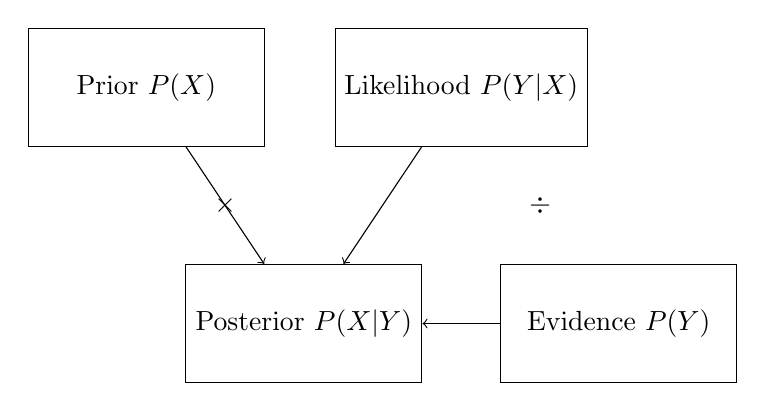
\begin{tikzpicture}
\node[draw, rectangle, minimum width=3cm, minimum height=1.5cm] (prior) at (0,0) {Prior $P(X)$};
\node[draw, rectangle, minimum width=3cm, minimum height=1.5cm] (likelihood) at (4,0) {Likelihood $P(Y|X)$};
\node[draw, rectangle, minimum width=3cm, minimum height=1.5cm] (posterior) at (2,-3) {Posterior $P(X|Y)$};
\node[draw, rectangle, minimum width=3cm, minimum height=1.5cm] (evidence) at (6,-3) {Evidence $P(Y)$};

\draw[->] (prior) -- (posterior);
\draw[->] (likelihood) -- (posterior);
\draw[->] (evidence) -- (posterior);

\node at (1,-1.5) {$\times$};
\node at (5,-1.5) {$\div$};
\end{tikzpicture}
\caption{Bayes' theorem as a belief update process}
\label{fig:bayes-process}
\end{figure}

The formula can be read as: "Posterior = (Likelihood × Prior) ÷ Evidence"

\subsection{Application to Machine Learning}

Bayes' theorem forms the basis of:
\begin{itemize}
    \item Bayesian inference
    \item Naive Bayes classifiers
    \item Maximum a posteriori (MAP) estimation
    \item Bayesian neural networks
\end{itemize}

Given data $\mathcal{D}$ and model parameters $\theta$:

\begin{equation}
P(\theta|\mathcal{D}) = \frac{P(\mathcal{D}|\theta)P(\theta)}{P(\mathcal{D})}
\end{equation}
